% \documentclass[10pt]{sosp2015}
% \documentclass[10pt,onecolumn]{sosp2015}
\documentclass[10pt,onecolumn,letterpaper]{article}
% \usepackage[10pt,inchmargins]{sigmin}  %% template from Xi Wang.
%\special{papersize=8.5in,11in}
%\setlength{\pdfpagewidth}{8.5in}
%\setlength{\pdfpageheight}{11in}
\usepackage[noheadfoot,
	      left=1in,right=1in,top=1in,bottom=1in,
             columnsep=0.3in
             ]{geometry}
\usepackage[small,compact]{titlesec}
\usepackage[font={small,bf}]{caption}    % added 9/10/13
\usepackage[nolineno,noindent,norules]{lgrind}
\usepackage{tightenum}
\usepackage{float}
\usepackage{xspace}
\usepackage{times,pifont}
\usepackage{mathptmx}
\usepackage{subfig,graphics,graphicx,color}
\usepackage{multirow}
\usepackage{dblfloatfix} %% correctly orders single- and double-col figures
\usepackage{hyphenat}
\usepackage{mathrsfs}
\usepackage{subfig}
\usepackage{amssymb,amsmath,centernot}
\usepackage{lastpage}
\usepackage{flushend}
\usepackage{hhline}
\usepackage{authblk}
%\newcommand{\doi}{XXXXXX}


%%% ================= START of SOSP '13 template ================= 
% \makeatletter
% 
% \def\ftype@copyrightbox{8}
% \def\@copyrightspace{
% \@float{copyrightbox}[b]
% \begin{center}
% \setlength{\unitlength}{1pc}
% \begin{picture}(20,6.0) 
% \put(0,3){\parbox{\columnwidth}{\scriptsize
% 
% %*** SAMPLE. AUTHOR PUT SUPPLIED TEXT HERE ****
% 
% \noindent
% \rule{6.0 cm}{0.2pt}\\
% Permissiondddd to make digital or hard copies of part or all of this work 
% for personal or classroom use is granted without fee provided that
% copies are not made or distributed for profit or commercial advantage 
% and that copies bear this notice and the full citation on the first
% page. Copyrights for third-party components of this work must be
% honored.  For all other uses, contact the Owner/Author. 
% 
% \vspace{\baselineskip}\noindent
% Copyright is held by the Owner/Author(s).\\
% \textit{SOSP'15}.\\
% ACM XXXXXXX.
% 
% \noindent
% http://dx.doi.org/\doi}
% }
% \end{picture}
% \end{center}
% \end@float}
% 
% \def\maketitle{\par
%  \begingroup
%    \def\thefootnote{\fnsymbol{footnote}}
%    \def\@makefnmark{\hbox
%        to 0pt{$^{\@thefnmark}$\hss}}
%      \twocolumn[\@maketitle]
% \@thanks
%  \endgroup
%  \setcounter{footnote}{0}
%  \let\maketitle\relax
%  \let\@maketitle\relax
%  \gdef\@thanks{}\gdef\@author{}\gdef\@title{}\gdef\@subtitle{}\let\thanks\relax
%  \@copyrightspace}
% 
% \makeatother

%%% ================= END of SOSP '13 template ================= 



%\newcommand{\comment}[1]{}
\frenchspacing

%\doublespacing

%%%%%%%%%%%%%%%%%%%%%%%%%%%%
%     macro

\newcommand{\xxx}[0]{\textsc{APUS}\xspace}
\newcommand{\yyy}[0]{\textsc{PLOVER}\xspace}
\newcommand{\paxos}[0]{\textsc{Paxos}\xspace}
\newcommand{\mytitle}[0]{\textbf {\xxx: Fast and Scalable \paxos on RDMA}}
\newcommand{\mykeywords}[0]{State Machine Replication, Fault Tolerance, Stable 
and Deterministic Multithreading, Software Reliability}

%%%%%%%%%%%%%%%%%%%%%%%%%%%%%%%%%%%%%%%%%%%%%%%%%%%%%%%%%%%%%%%%%
% hyperref stuff

%\usepackage[square,comma,numbers,sort]{natbib}
\usepackage{hypernat}
\usepackage{hyperref}

%% fill in pdf info here
\hypersetup{%
colorlinks=false,
pdfborder={0 0 0},
pdftitle={\mytitle},
pdfkeywords={\mykeywords},
bookmarksnumbered,
pdfstartview={FitH},
urlcolor=cyan,
pdfpagelabels=true,
pdfdisplaydoctitle=true,
}%

%\usepackage{breakurl}
%\usepackage[all]{hypcap}
%\renewcommand{\url}{\burl}

%%%%%%%%%%%%%%%%%%%%%%%%%%%%%%%%%%%%%%%%%%%%%%%%%%%%%%%%%%%%
% Some NICE fonts

\newfont{\BIG}{cminch}                             %--- One-inch font
\newfont{\sfbHuge}{cmssbx10 scaled\magstep5}       %-- 25pt sans serif bold
\newfont{\sfbLarger}{cmssbx10 scaled\magstep3}   %-- 12+pt sans serif boldd
\newfont{\sfblarger}{cmssbx10 scaled\magstep2}   %-- 12+pt sans serif bold
\newfont{\sfblarge}{cmssbx10 scaled\magstep1}      %-- 12pt sans serif bold
\newfont{\sfbeleven}{cmssbx10 scaled\magstephalf}  %-- 11pt sans serif bold
\newfont{\sfb}{cmssbx10}                           %-- 10pt sans serif bold
\newfont{\sfeight}{cmss8}                          %-- 8pt sans serif

%%%%%%%%%%%%%%%%%%%%%%%%
%    space tweaking

%\textwidth = 6.5 in
%\textheight = 9.0 in
%\setlength{\topmargin}{-.5in}

%\headheight = 0.0 in
%\headsep = 0.0 in
%\parskip = 0.2in
%\parindent = 0.0in

\renewcommand{\topfraction}{0.95}
\addtolength{\textfloatsep}{-0.1in}
%\addtolength{\floatsep}{0.025in}
\renewcommand\floatpagefraction{.9}
%\renewcommand\bottomfraction{.9}
\renewcommand\textfraction{.1}

\setlength{\parindent}{9pt}

% Rescue
\makeatletter
\def\v#1{{\mbox{\fontfamily{cmtt}\fontsize{\f@size}{\f@size}\selectfont #1}}}

\newcommand{\dmt}[0]{DMT\xspace}
\newcommand{\smt}[0]{StableMT\xspace}
\newcommand{\smr}[0]{SMR\xspace}

\newcommand{\racepro}[0]{\textsc{RacePro}\xspace}
\newcommand{\criu}[0]{\textsc{CRIU}\xspace}
\newcommand{\lxc}[0]{\textsc{LXC}\xspace}
\newcommand{\tern}[0]{\textsc{Tern}\xspace}
\newcommand{\peregrine}[0]{\textsc{Peregrine}\xspace}
\newcommand{\parrot}[0]{\textsc{Parrot}\xspace}
\newcommand{\repframe}[0]{\textsc{RepFrame}\xspace}
\newcommand{\grace}[0]{Grace\xspace}
\newcommand{\coredet}[0]{\textsc{CoreDet}\xspace}
\newcommand{\kendo}[0]{Kendo\xspace}
\newcommand{\dthreads}[0]{\textsc{DThreads}\xspace}
\newcommand{\determinator}[0]{Determinator\xspace}
\newcommand{\dos}[0]{dOS\xspace}
\newcommand{\ddos}[0]{DDOS\xspace}
\newcommand{\timealgo}[0]{time bubbling\xspace}
\newcommand{\ldpreload}[0]{LD\_PRELOAD\xspace}
\newcommand{\ntimeout}[0]{$W_{timeout}$\xspace}
\newcommand{\nclock}[0]{$N_{clock}$\xspace}
\newcommand{\us}[0]{\(\mu\text{s}\)\xspace}

\newcommand{\apache}{\v{Apache}\xspace}
\newcommand{\mongoose}[0]{\v{Mongoose}\xspace}
\newcommand{\ab}{\v{ApacheBench}\xspace}
\newcommand{\clamav}{\v{ClamAV}\xspace}
\newcommand{\upnp}{uPnP\xspace}
\newcommand{\mediatomb}{\v{MediaTomb}\xspace}
\newcommand{\mencoder}{\v{mencoder}\xspace}
\newcommand{\mongodb}{\v{MongoDB}\xspace}
\newcommand{\ssdb}{\v{SSDB}\xspace}
\newcommand{\mysql}{\v{MySQL}\xspace}
\newcommand{\sysbench}{\v{SysBench}\xspace}
\newcommand{\zookeeper}{\v{ZooKeeper}\xspace}
\newcommand{\dare}{\v{DARE}\xspace}

\newcommand{\calvin}{\v{Calvin}\xspace}
\newcommand{\libpaxos}{libPaxos\xspace}
\newcommand{\crane}{\textsc{Crane}\xspace}
\newcommand{\nopaxos}{NOPaxos\xspace}
\newcommand{\spaxos}[0]{S-Paxos\xspace}
\newcommand{\nkvprog}[0]{4\xspace}
\newcommand{\memcached}{\v{Memcached}\xspace}
\newcommand{\comptradlow}[0]{32.3X\xspace}
\newcommand{\tputoverhead}[0]{4.2\%\xspace}
\newcommand{\latencyoverhead}[0]{4.3\%\xspace}
\newcommand{\fasterDARE}[0]{4.9X\xspace}

\newcommand{\pgsql}{\v{PgSql}\xspace}
\newcommand{\tomcat}{\v{Tomcat}\xspace}
\newcommand{\qemumc}[0]{MC\xspace}
\newcommand{\remus}[0]{\textsc{Remus}\xspace}
\newcommand{\colo}[0]{\textsc{Colo}\xspace}
\newcommand{\vsmr}[0]{VSMR\xspace}
\newcommand{\nginx}{\v{Nginx}\xspace}
\newcommand{\python}{Python\xspace}
\newcommand{\php}{PHP\xspace}
\newcommand{\jsp}{JSP\xspace}
\newcommand{\cms}[0]{DjCMS\xspace}
\newcommand{\kvm}[0]{KVM\xspace}
\newcommand{\ms}[0]{ms\xspace}
\newcommand{\avgtput}[0]{2.1X\xspace}
\newcommand{\avgbandwidth}[0]{12.2X\xspace}
\newcommand{\avgsixteen}[0]{4.3X\xspace}

\newcommand{\aget}[0]{\v{aget}\xspace}
\newcommand{\pthread}[0]{\mbox{Pthreads}\xspace}
\newcommand{\openldap}[0]{{OpenLDAP}\xspace}
\newcommand{\redis}[0]{{Redis}\xspace}
\newcommand{\bdb}[0]{{Berkeley DB}\xspace}
\newcommand{\vtune}[0]{\v{VTune}\xspace}
\newcommand{\http}[0]{\mbox{HTTP}\xspace}

% In short.
\newcommand{\eg}{{e.g.}}
\newcommand{\ie}{{i.e.}}
\newcommand{\etc}{{etc}}
\newcommand{\para}[1]{\vspace{.00in}\noindent{\bf #1}}
\newcommand{\wrt}{{w.r.t. }}
\newcommand{\cf}{{cf. }}

% Synch and network operations.
\newcommand{\checktimebubble}[0]{\v{check\_add\_timebubble()}\xspace}
\newcommand{\mutexlock}[0]{\v{pthread\_mutex\_lock()}\xspace}
\newcommand{\connect}[0]{\v{connect()}\xspace}
\newcommand{\send}[0]{\v{send()}\xspace}
\newcommand{\sendto}[0]{\v{sendto()}\xspace}
\newcommand{\sendmsg}[0]{\v{sendmsg()}\xspace}
\newcommand{\mywrite}[0]{\v{write()}\xspace}
\newcommand{\pwrite}[0]{\v{pwrite()}\xspace}
\newcommand{\close}[0]{\v{close()}\xspace}
\newcommand{\recv}[0]{\v{recv()}\xspace}
\newcommand{\select}[0]{\v{select()}\xspace}
\newcommand{\poll}[0]{\v{poll()}\xspace}
\newcommand{\epollwait}[0]{\v{epoll\_wait()}\xspace}
\newcommand{\accept}[0]{\v{accept()}\xspace}

% Parrot primitives.
\newcommand{\getturn}[0]{\v{get\_turn()}\xspace}
\newcommand{\putturn}[0]{\v{put\_turn()}\xspace}
\newcommand{\wait}[0]{\v{wait()}\xspace}
\newcommand{\signal}[0]{\v{signal()}\xspace}

% Evaluation stats.
\newcommand{\github}[0]{\url{github.com/columbia/crane}}
% \newcommand{\ntype}[0]{four\xspace}
\newcommand{\nprog}[0]{nine\xspace}
\newcommand{\overheadmax}[0]{22.99\%\xspace}
\newcommand{\overhead}[0]{34.19\%\xspace}
\newcommand{\dmtspeedup}[0]{10.5\%\xspace}
\newcommand{\proxyoverhead}[0]{2.33\%\xspace}
\newcommand{\timebubblelow}[0]{66.65\%\xspace}
\newcommand{\timebubblehigh}[0]{93.88\%\xspace}
\newcommand{\recovertime}[0]{1.97ms\xspace}
\newcommand{\downgradetime}[0]{0.36s\xspace}
\newcommand{\mencoderspeedup}{\v{49\%}\xspace}

\def\LGfsize{\footnotesize}
%\pagestyle{empty}


% \conferenceinfo{SOSP'15}{October 4--7, 2015, Monterey, CA}
% \copyrightyear{2015} 
% \copyrightdata{978-1-4503-3834-9/15/10} 
% \doi{2815400.2815427}

\title{\mytitle}
% \authorinfo{Authors}

% \author[+*]{Heming Cui}
% \author[*]{Rui Gu}
% \author[*]{Cheng Liu}
% \author[x]{Tianyu Chen}
% \author[*]{Junfeng Yang}
% \setlength{\affilsep}{0.5em}
% \renewcommand\AB@affilsepx{\hspace{28.0 mm}\protect\Affilfont}
% \affil[+]{\textrm\fontsize{10}{10}\selectfont The University of Hong Kong}
% \affil[*]{\textrm Columbia University}
% \affil[x]{\textrm Tsinghua University\vspace{-7.0 mm}}

\begin{document}

% Hack for: Package caption Error: No float type 'copyrightbox' defined.
%\newcounter{copyrightbox}

\date{}

\author[+]{}
\maketitle
%\thispagestyle{empty}

% \begin{sloppypar}
% \begin{abstract}
% \input{abstract}
% \end{abstract}
% \end{sloppypar}

% \begin{sloppypar}
%% %\category{D.2.5}{Software Engineering}{Testing and Debugging}
%% \category{D.4.5}{Operating Systems}{Threads, Reliability}
%% \category{D.2.4}{Software Engineering}{Software/Program Verification}
%% \terms{Algorithms, Design, Reliability, Performance}
%% \keywords{\mykeywords}

%% \vskip 2mm
%% \noindent {\small \bf Categories and Subject Descriptors:} \vskip -.2mm
%% \noindent
%% {\footnotesize D.4.5~[{\bf Operating Systems}]: {Threads, Reliability}\\
%% D.2.4~[{\bf Software Engineering}]: {Software/Program Verification};}
%% \vskip 1mm
%% \noindent {\small \bf General Terms:} \vskip -.2mm
%% \noindent
%% {\footnotesize Algorithms, Design, Reliability, Performance}
%% \vskip 1mm
%% \noindent {\small \bf Keywords:} \vskip -.2mm
%% \noindent
%% {\footnotesize \mykeywords}

% \vskip 2mm
% \noindent {\small \bf Categories and Subject Descriptors:}
% {\small D.4.5~[{\bf Operating Systems}]: {Threads, Reliability};
%   D.2.4~[{\bf Software Engineering}]: {Software/Program Verification};}
% \vskip .1mm
% \noindent {\small \bf General Terms:} {\small Algorithms, Design,
%   Reliability, Performance}
% \vskip .1mm
% \noindent {\small \bf Keywords:} {\small \mykeywords}
% 
% \end{sloppypar}

%%%%%%%%%%%%%%%%%%%%%%%%%%%%%%%%%%%
% Add page number.
\setcounter{page}{1}
\pagenumbering{arabic}

\thispagestyle{plain}
\pagestyle{plain}
\setlength{\footskip}{20pt}
%%%%%%%%%%%%%%%%%%%%%%%%%%%%%%%%%%%

% \begin{sloppypar}
% 
% \vskip 2mm
% \noindent {\small \bf Categories and Subject Descriptors:}
% {\small D.4.5~[{\bf Operating Systems}]: {Threads, Reliability};
%   C.2.4~[{\bf Computer-communication Networks}]: {Distributed Systems};}
% \vskip .1mm
% \noindent {\small \bf General Terms:} {\small Algorithms, Design,
%   Reliability, Performance}
% \vskip .1mm
% \noindent {\small \bf Keywords:} {\small \mykeywords}
% 
% \end{sloppypar}

\begin{sloppypar}
\section{Introduction} \label{sec:intro}
Existing \paxos protocols suffer from high, scale-limited consensus latency. OS 
kernel, a major source of this problem, can be bypassed with advanced network 
features such as Remote Direct Memory Access (RDMA) within the same datacenter.

In this report, we present \xxx, an RDMA-based \paxos protocol and its runtime 
system that can efficiently provide fault tolerance to unmodified server 
programs. \xxx intercepts an unmodified server program's inbound socket calls 
(\eg, \recv), assigns a total order for all received requests in all 
connections, and uses fast RDMA primitives to invoke consensus on these requests 
concurrently. To ensure the same robustness as regular \paxos, \xxx's runtime 
system efficiently tackles several reliability challenges such as atomic 
delivery of messages (\S\ref{sec:atomic}).
\section{Background on RDMA}\label{sec:background}

RDMA is a kernel-bypassing technique that offers ultra low latency and high 
throughput. As the prices decrease, RDMA architectures (\eg, 
Infiniband~\cite{infiniband} and RoCE~\cite{roce}) have become common within a 
datacenter.

RDMA has three operation types, from fast to slow: one-sided 
read/write operations, two sided send/recv operations. An one-sided RDMA write 
can directly write from one replica's memory to a remote replica's memory 
without involving the remote OS kernel or CPU. Prior work~\cite{pilaf:usenix14} 
shows that one-sided operations are up to 2X faster than two-sided 
operations~\cite{fasst:osdi16}, so \xxx uses one-sided operations (or ``WRITE" 
in this report). On a WRITE success, the remote NIC (network interface card) 
sends an RDMA ACK to local NIC.

A one-sided RDMA communication between a local and a remote NIC has
a Queue Pair (QP), including a send queue and a receive 
queue. Such a QP is a global data structure between every two replicas, but 
pushing a message into a local QP takes at most 0.2 \us in our evaluation. 
Different QPs between different replicas work in parallel (leveraged by \xxx in 
\S\ref{sec:normal}). Each QP has a Completion Queue (CQ) to store ACKs. A QP 
belongs to a type of ``XY": X can be R (reliable) or U (unreliable), and Y can 
be C (connected) or U (unconnected). HERD~\cite{herd:sigcomm14} shows that 
WRITEs on RC and UC QPs incur almost the same latency, so \xxx uses RC QPs.

Normally, to ensure a WRITE resides in remote memory, the local replica 
busily polls an ACK from the CQ before it proceeds 
(or \emph{signaling}). Polling ACK is time consuming as it involves 
synchronization between the NICs on both sides of a CQ. We looked into the ACK 
pollings in a recent RDMA-based consensus protocol \dare~\cite{dare:hpdc15}.
We found that, although it is highly optimized (its leader maintains one 
global CQ to receive all backups' ACKs in batches), busily polling ACKs slowed 
\dare down: when the CQ was empty, each poll took 0.039$\sim$0.12 \us; when the 
CQ has one or more ACKs, each poll took 0.051$\sim$0.42 \us.

Fortunately, depending on protocol logic, one can do \emph{selective 
signaling}~\cite{herd:sigcomm14}: it only checks for an ACK after pushing a 
number of WRITEs. Because \xxx's protocol logic does not rely on RDMA ACKs, 
it just occasionally invokes selective signaling to clean up ACKs.
\section{Overview} \label{sec:overview}

We present \xxx, an RDMA-based fault tolerance system that can efficiently 
replicate unmodified server programs. \xxx intercepts an unmodified server 
program's inbound socket calls (\eg, \recv), assigns a total order for all 
received requests in all connections, and uses fast RDMA primitives to invoke 
consensus on these requests concurrently. To ensure the same robustness as 
regular \paxos, \xxx's runtime system efficiently tackles several reliability 
challenges such as atomic delivery of messages (\S\ref{sec:atomic}).

\subsection{Architecture} \label{sec:arch}

\xxx deployment is similar to a typical State Machine Replication (\smr) 
system: it runs a server program on replicas within a datacenter. Replicas 
connect with each other using RDMA QPs. Client programs are located in LAN or 
WAN.

\begin{figure*}[ht]
\begin{center}
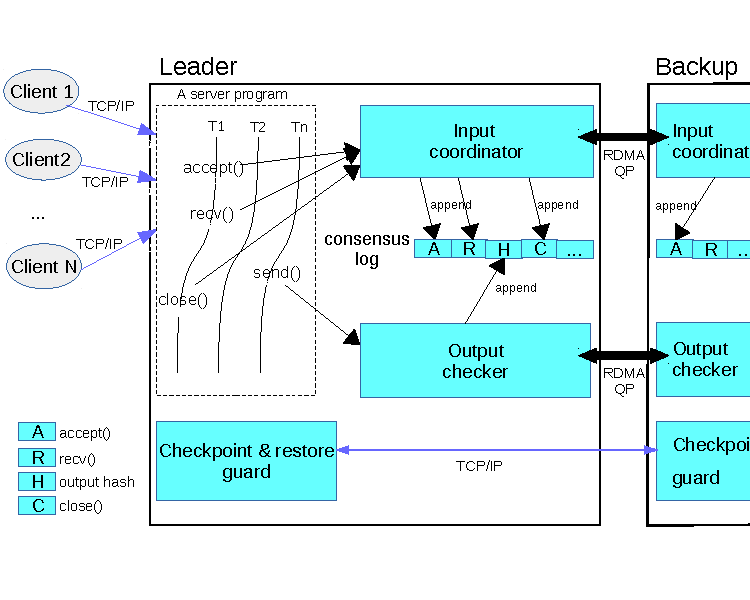
\includegraphics{figures/arch}
\caption{\em \xxx Architecture (key components are in
  blue).}\label{fig:arch}
\end{center}
\end{figure*}

The \xxx leader handles client requests and runs its RDMA-based protocol to 
enforce the same total order for all requests across replicas.

Figure~\ref{fig:arch} shows \xxx's architecture. \xxx intercepts a server 
program's inbound socket calls (\eg, \recv) using a Linux technique called 
\ldpreload. \xxx involves four key components: a \paxos consensus protocol for 
input coordination (in short, the \emph{coordinator}), a circular in-memory 
consensus log (the \emph{log}), a guard process that handles checkpointing 
and recovering a server's process and file system state (the 
\emph{guard}), and an optional output checking tool (the \emph{checker}).

The coordinator is involved when a thread of a program running on the \xxx 
leader calls an inbound socket call (\eg, \recv). The thread executes the 
Libc call, gets the received data, appends a log entry on the leader's local 
consensus log, and replicates this entry to backups' consensus logs using our 
\paxos protocol (\S\ref{sec:protocol}).

In this protocol, all threads in the server program running on the leader 
replica can concurrently invoke consensus on their log entries (requests), but 
\xxx enforces a total order for all entries in the leader's local consensus 
log. As a consensus request, each thread does an RDMA WRITE to replicate its 
log entry to the corresponding log entry position on all \xxx backups. Each 
\xxx backup polls from the latest unagreed entry on its local consensus log; 
if it agrees with the proposed log entry, it does an RDMA WRITE to write a 
consensus reply on the leader's corresponding entry.

To ensure \paxos safety~\cite{paxos:practical}, all \xxx backups agree on the 
entries proposed from the leader in a total order without allowing any entry 
gap. When a majority of replicas (including the leader) has written a consensus 
reply on the leader's local entry, this entry has reached a consensus. By doing 
so, \xxx consistently enforces the same consensus log for both the leader and
backups.

The output checker is periodically invoked as a program replicated in \xxx 
executes outbound socket calls (\eg, \send). For every 1.5KB (MTU size) of 
accumulated outputs per connection, the checker unions the previous hash with 
current outputs and computes a new CRC64 hash. For simplicity, the output 
checker uses \xxx's input consensus protocol (\S\ref{sec:protocol}) to compare 
hashes across replicas.

\section{Protocol} \label{sec:protocol}

\subsection{Normal Case} \label{sec:normal}
\xxx's consensus protocol has three main elements. 
First, a \paxos consensus log. Second, threads of a server program running on 
the leader host (or \emph{leader threads}). \xxx hooks the inbound socket calls 
(\eg, \recv) of these leader threads and invoke consensus requests on these 
calls. We denote the data received from each of these calls as a consensus 
request (\ie, an entry in the consensus log). Third, a \xxx internal thread 
running on every backup (or \emph{backup threads}), which agrees on consensus 
requests. The \xxx leader enables the first and second elements, and backups 
enable the first and third elements.

\begin{figure}[h]
\begin{minipage}{3in}
\lgrindfile{code/logentry.cpp}
\end{minipage}
\caption{{\em \xxx's log entry for each socket call.}}
\label{fig:logentry}
\end{figure}

Figure~\ref{fig:logentry} depicts the format of a log entry in \xxx's consensus 
log. Most fields are the same as those in a typical \paxos 
protocol~\cite{paxos:practical} except three: the \v{reply} array, 
\v{conn\_vs}, and \v{call\_type}. 
The \v{reply} array is a piece of memory on the leader side, preserved for
backups to do RDMA WRITEs for their consensus replies. 
%is for backups to do RDMA WRITEs for their 
%consensus replies on the leader. 
The \v{conn\_vs} is for identifying
which TCP connection this socket call belongs to (see \S\ref{sec:concurrent}). 
The \v{call\_type} identifies different types of socket calls (\eg, the \accept 
type and the \recv type) for the entry.

% Second, leader thread behavior on \recv(). Return from orig recv, grab 
% spin % lock and get view stamp, store the log, and post send to all replicas. 
% Non blocking. Wait % for over half agree, and then execute the operation.
Figure~\ref{fig:consensus} shows \xxx's consensus protocol. Suppose a leader 
thread invokes a consensus request when it calls a socket call \recv. This 
thread's consensus request has four steps. The first step (\textbf{L1}, not 
shown in Figure~\ref{fig:consensus}) is executing the actual socket call, 
because the thread needs to get the received data and returned value, to 
allocate a distinct log entry, and to replicate the entry in backups' consensus 
logs.

The second step (\textbf{L2}) is local preparation, including assigning a 
viewstamp (a totally-ordered \paxos consensus request 
ID~\cite{paxos:practical}) 
for this entry in the consensus log, allocating a distinct entry in the log, 
and 
storing the entry to a local storage. We denote the time 
taken on storing an entry as $t_{SSD}$. 
% without allowing gaps (\ig, newer 
% entries reach consensus but ).

Third, each leader thread concurrently invokes a consensus via the third step 
(\textbf{L3}): WRITE the log entry to remote backups. This step is thread-safe 
because each leader thread works on its own distinct entry and remote backups' 
corresponding entries. An \textbf{L3} WRITE returns quickly after 
pushing the entry to its local QP connecting the leader and each backup. We 
denote the time taken for this push as $t_{PUSH}$, which took at most 0.2\us in 
our evaluation. $t_{PUSH}$ is serial for concurrently arriving requests 
on each QP, but the WRITEs (all \textbf{L3} arrows in 
Figure~\ref{fig:logentry}) to different QPs run in parallel.

The fourth step (\textbf{L4}) is that the leader thread polls on its 
\v{reply} field in its local log entry to wait for backups' consensus replies. 
It breaks the poll if a number of heartbeats fail 
(\S\ref{sec:election}). If a majority of replicas agrees on the entry, an input 
consensus is reached, the 
leader thread leaves this \recv call and proceeds with its program logic.

\begin{figure*}[ht]
\begin{center}
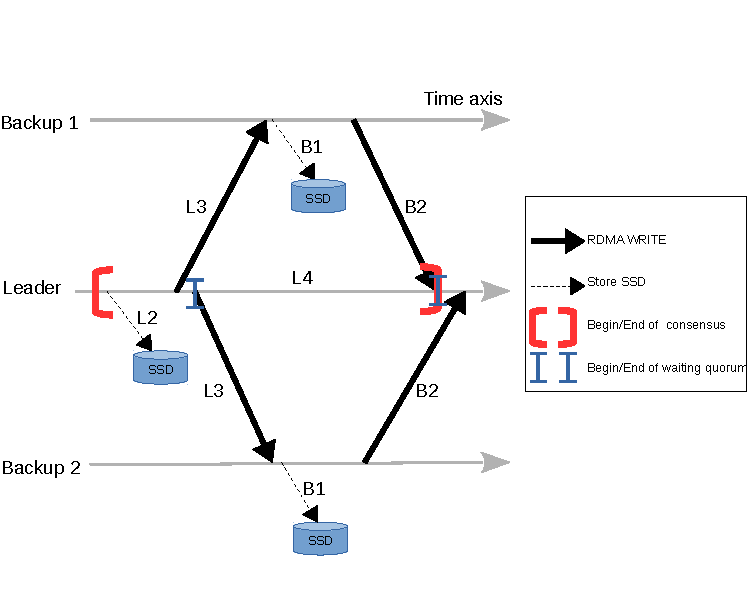
\includegraphics{figures/consensus}
\caption{\em \xxx consensus algorithm in normal case.}\label{fig:consensus}
\end{center}
\end{figure*}

On each backup, a backup thread polls from the latest unagreed log entry. It 
breaks the poll if a number of heartbeats fail 
(\S\ref{sec:election}). 
If no heartbeat fails, the backup thread then agrees on entries in the same 
total order as those on the leader's consensus log, using three steps. First 
(\textbf{B1}), it does a regular \paxos view ID check~\cite{paxos:practical} to 
see whether the leader's view ID matches its own one, it then stores the log 
entry in its local SSD. To scale to concurrently arriving requests, the backup 
thread scans multiple entries it agrees with at once. It then stores them 
in \xxx's parallel storage.

Second (\textbf{B2}), on each entry the backup agrees, the backup thread does 
an RDMA WRITE to send back a consensus reply to the \v{reply} array element in 
the leader's corresponding entry. Third (\textbf{B3}, not shown 
in Figure~\ref{fig:consensus}), the backup thread does a regular \paxos 
check~\cite{paxos:practical} on \v{last\_committed} and to know the latest 
entry that has reached consensus. It then ``executes" the committed entries by 
forwarding the data in these entries to the server program on its local 
replica. Carrying latest committed entries in next consensus requests is a 
common, efficient \paxos implementation method~\cite{paxos:practical}.

To ensure \paxos safety, the backup thread agrees on log 
entries in order without allowing any gap~\cite{paxos:practical}. If the 
backup suspects it misses some log entries (\eg, because of packet loss),
it invokes a learning request to the leader asking for the 
missing entries.

\subsection{Atomic Message Delivery} \label{sec:atomic}

% One key issue, check integrity. Strawmen approach, check viewstamp first.
On a backup side, one tricky challenge is that atomicity must be 
ensured on the leader's RDMA WRITEs on all entries and backups' polls. For 
instance, while a leader thread is doing a WRITE on \v{vs} to a remote backup, 
the backup's thread may be reading \v{vs} concurrently, causing a 
corrupted read value.

To address this challenge, one prior 
approach~\cite{farm:nsdi14,herd:sigcomm14} 
leverages the left-to-right ordering of RDMA WRITEs and puts a special 
non-zero variable at the end of a fix-sized log entry because they mainly 
handle key-value stores with fixed value length. As long as this variable is 
non-zero, the RDMA WRITE ordering guarantees that the log entry WRITE is 
complete. However, because \xxx aims to support general server programs with 
largely variant received data lengths, this approach cannot be applied in \xxx.

Another approach is using atomic primitives provided by RDMA hardware, 
but a prior evaluation~\cite{drtm:sosp15} has shown that RDMA atomic 
primitives are much slower than normal RDMA WRITEs and local memory reads.

\xxx tackles this challenge by using the leader to add a canary value after 
the \v{data} array. A backup thread always first checks the canary value 
according to \v{data\_size} and then starts a standard \paxos consensus 
reply decision~\cite{paxos:practical}. This synchronization-free approach 
ensures that a \xxx backup thread always reads a complete entry efficiently.

\subsection{Handling Concurrent Connections} \label{sec:concurrent}

Unlike traditional \paxos protocols which mainly handle single-threaded 
programs due to the deterministic execution assumption in \smr, \xxx aims 
to support both single-threaded as well as multi-threaded or -processed 
programs running on multi-core machines. Therefore, a strongly consistent 
mechanism is needed to map each connection on the leader and 
its corresponding connection on backups. A naive approach is matching a 
leader connection's socket descriptor to the same one on a backup, but programs 
on backups may return nondeterministic descriptors due to systems resource 
contention.

Fortunately, \paxos already makes viewstamps~\cite{paxos:practical} of 
requests (log entries) strongly consistent across replicas. For TCP 
connections, \xxx adds the \v{conn\_vs} field, the viewstamp of the the first 
socket call in each connection (\ie, \accept) as the connection ID for log 
entries.

\subsection{Leader Election} \label{sec:election}

Leader election on RDMA raises a main challenge: because backups do not 
communicate with each other in normal case, a backup proposing itself as 
the new leader does not know the remote memory locations where the other 
backups are polling. Writing to a wrong remote memory location may cause the 
other backups to miss all leader election messages. A recent 
system~\cite{dare:hpdc15} establishes an extra control QP to handle leader 
election, complicating deployments.

\xxx addresses this challenge with a simple, clean design. It runs leader 
election on the normal-case consensus log and QP. In normal case, the 
leader does WRITEs to remote logs as heartbeats with a period of T. Each 
consensus log maintains an \v{elect[MAX]} array, one array
element for each replica. This \v{elect} array is only used in leader election. 
Once backups miss heartbeats from the leader for 3*T, they suspect the leader 
to fail, close the leader's QPs, and start to work on the \v{elect} array to 
elect a new leader.

Backups use a standard \paxos leader election algorithm~\cite{paxos:practical} 
with three steps. Each backup writes to its own \v{elect} element indexed by 
its replica ID on other replicas' \v{elect}. First, each backup waits for a 
random time (similar to random election timeouts in Raft~\cite{raft:usenix14}), 
and it proposes a new view with a standard two-round 
\paxos consensus~\cite{paxos:simple} by including both its view and the index 
of its latest log entry. The other backups also propose their views and poll on 
this \v{elect} array in order to agree on an earlier proposal or confirm itself 
as the winner. The backup with a more up-to-date log will win the proposal. A 
log is more up-to-date if its latest entry has either a higher view or the same 
view but a higher index.

Second, the winner proposes itself as a leader candidate using this \v{elect}
array. Third, after the second step reaches a quorum, the new leader notifies 
remote replicas itself as the new leader and it starts to WRITE periodic 
heartbeats. Overall, \xxx safely avoids multiple ``leaders" to corrupt 
consensus logs, because only one leader is elected in each view, and backups 
always close an outdated leader's QPs before electing a new leader. For 
robustness, the above three steps are inherited from a practical \paxos 
election algorithm~\cite{paxos:practical}, but \xxx makes the election 
efficient and simple in an RDMA domain.
\section{Initial Results} \label{sec:evaluation}
We implemented the normal case of our protocol and collected initial 
results.

Evaluation was done on nine RDMA-enabled Dell R430 and five Supermirco 
SuperServer 1019P hosts. Each host has Linux 3.16.0 and 2.6 GHz Intel Xeon 
CPU. The Dell R430 hosts are equipped with 24 hyperthreading cores, 64 GB 
memory, and 1 TB SSD. The SuperServer 1019P hosts have 28 hyperthreading 
cores, 32 GB memory, and 375GB SSD. All NICs are Mellanox ConnectX-3 (40Gbps) 
connected with RoCE~\cite{roce}.

We compared \xxx with five open source consensus protocols, including four 
traditional ones (\libpaxos~\cite{libpaxos}, \zookeeper~\cite{zookeeper}, 
\crane~\cite{crane:sosp15} and \spaxos~\cite{spaxos:srds12}).

We evaluated \xxx on \nprog widely used or studied programs, including
\nkvprog key-value stores \redis, \memcached, \ssdb, \mongodb; \mysql, a SQL
server; \clamav, an anti-virus server that scans files and delete malicious 
ones; \mediatomb, a multimedia storage server that stores and transcodes video 
and audio files; \openldap, an LDAP server; \calvin~\cite{calvin:sigmod12}, a 
popular \smr system for databases.

\subsection{Comparing w/ Traditional Consensus}
\label{sec:eval-traditional}

\begin{figure}[t]
\begin{center}
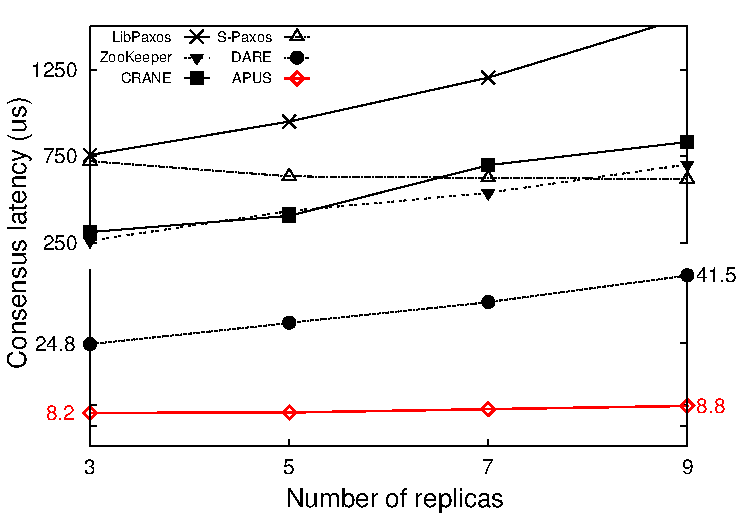
\includegraphics[width=3in]{figures/traditional_paxos_latency}
\caption{{\em Comparing \xxx to five existing consensus protocols.} All 
six protocols ran a client with 24 concurrent connections. The Y axis is 
broken to fit in all protocols.}
\label{fig:scalability}
\end{center}
\end{figure}

We ran \xxx and four traditional consensus protocols using their own 
client programs or popular client programs with 100K requests of similar sizes. 
For each protocol, we ran a client with 24 concurrent connections on a 24-core 
machine located in LAN, and we used up to nine replicas. Both the number of 
concurrent connections and replicas are common high 
values~\cite{zookeeper,crane:sosp15,rex:eurosys14,dare:hpdc15}.

Figure~\ref{fig:scalability} shows that the consensus latency of three 
traditional protocols increased almost linearly to the number of replicas 
(except \spaxos). \spaxos batches requests from replicas and invokes consensus 
when the batch is full. More replicas can take shorter time to form a batch, so 
\spaxos incurred a slightly better consensus latency with more replicas. 
Nevertheless, its latency was always over 600 \us. \xxx's consensus latency 
outperforms these four protocols by at least \comptradlow.

\subsection{Performance Overhead} \label{sec:overhead}

To stress \xxx, we used nine replicas to run all \nprog server 
programs without modifying them. We used up to 32 concurrent 
client connections (most evaluated programs reached peak throughput at 
16), and then we measured mean response time and throughput in 50 runs.

\begin{figure*}[t]
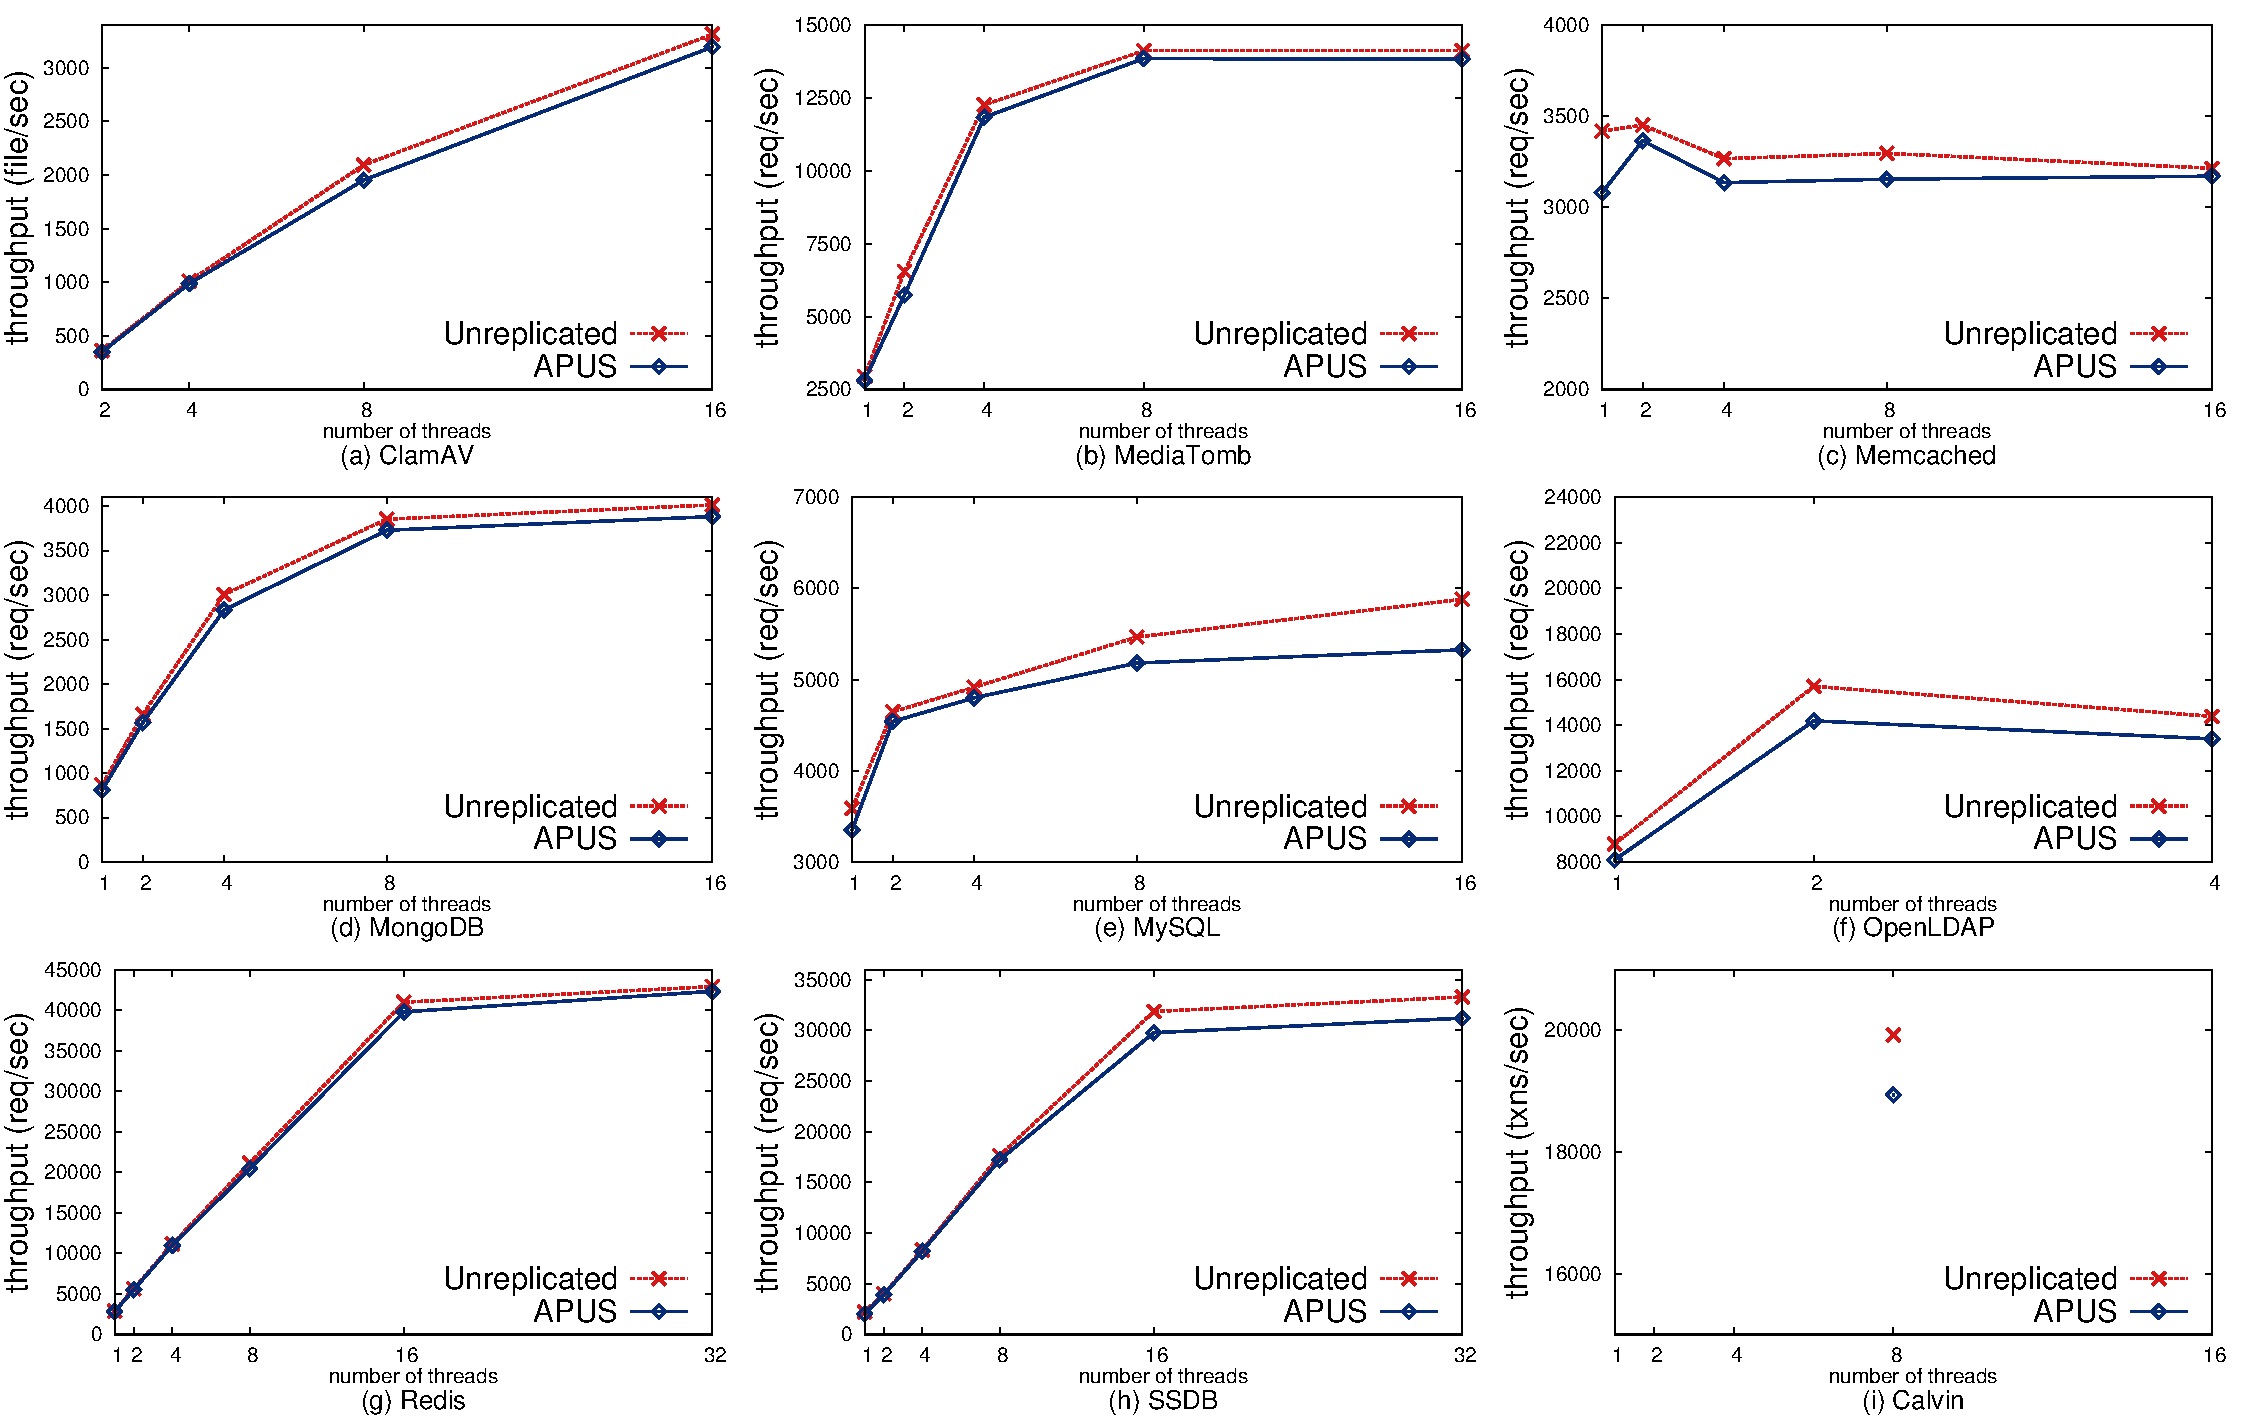
\includegraphics[width=6in]{figures/throughput}
\caption{\small {\em \xxx throughput compared to server programs' unreplicated
executions.}}
\label{fig:tput}
\end{figure*}

We turned on output checking and didn't 
observe a performance impact. Only two programs (\mysql and \openldap) 
have different output hashes caused by physical times 
(an approach~\cite{paxos:practical} can be leveraged to enforce same physical 
times across replicas).

Figure~\ref{fig:tput} shows \xxx's throughput. For \calvin, we only collected 
the 8-thread result because \calvin uses this constant thread count in their 
code to serve requests. Compared to these server programs' 
unreplicated executions, \xxx merely incurred a mean throughput overhead of 
\tputoverhead (note that in Figure~\ref{fig:tput}, the Y-axises of most 
programs start from a large number). As the number of threads increases, all 
programs' unreplicated executions got a performance improvement except 
\memcached. Prior work~\cite{rex:eurosys14} also showed that
\memcached itself scaled poorly. Overall, \xxx scaled as well as unreplicated 
executions on concurrent requests.

\subsection{Integrating \xxx into virtual machine} \label{sec:overhead}
Virtual machines usually use a primary-backup architecture for fault 
tolerance~\cite{alsberg1976principle}. However, primary-backup approach is 
notorious for the ``split-brain'' problem~\cite{scales2010design}, which can be 
avoided in \paxos. One reason for fault tolerant VMs to use 
primary-backup replication instead of \paxos protocol is that traditional \paxos 
systems incur high performance overhead. Specifically, every 
request received by the virtual machine must go through the traditional \paxos 
systems to reach consensus first, which takes hundreds of microseconds, and then 
be processed by the server programs. This high consensus latency severely 
degrades the performance of the applications running inside.

By integrating the fast \xxx \paxos protocol into virtual machine, we 
efficiently mitigate the ``split-brain'' problem caused by the primary-backup 
approach. We implemented the prototype on KVM QEMU hypervisor and it took fewer 
than ten lines of code by leveraging the simple API provided by \xxx.

\section{Integrating \xxx into virtual machine} \label{sec:vm-integration}

Primary-backup (\eg, \remus~\cite{remus:nsdi08}), a dominant Virtual Machine 
(VM) fault-tolerance approach, works in a physical time slot manner. In each 
slot, it runs a service in the primary VM to process client requests, tracks 
updated VM states (\eg, dirty memory pages), and buffers network outputs. 
At the end of a slot, a synchronization operation is invoked to transfer dirty 
pages from the primary to backup. Once the transfer succeeds, network outputs 
are sent to clients. By doing so, primary-backup approach ensures 
\emph{external consistency}~\cite{remus:nsdi08}: primary and backup have the 
same states and a primary failure will not be observed by clients.

Unfortunately, despite much effort~\cite{remus:nsdi08,qemu-mc, 
sartakov2017multi,lu2012speculative, gerofi2011rdma}, achieving fast and 
multi-core scalable VM fault-tolerance remains an open 
problem~\cite{dong2013colo,gerofi2011rdma,sartakov2017multi}. There are two main 
reasons for this. One is that the primary-backup approach often has to transfer 
an excessive amount of dirty memory pages, which greatly degrades the 
performance of a service and occupies prohibitive network bandwidth. The other 
reason is that primary-backup approach suffers from the notorious 
``split-brain'' problem~\cite{scales2010design}, in which both the primary and 
backup think itself as the primary when network partition happens and 
therefore break external consistency to the clients.

To address the problems mentioned above, we propose Virtualized \smr (\vsmr), a 
new \smr approach that can achieve fast, multi-core scalable VM fault-tolerance. 
\vsmr enforces same total order of network inputs for a VM replicated across 
hosts. It then periodically invokes a synchronization operation to efficiently 
compute updated page hashes, to compare them across the replicas, and to 
transfer only the divergent pages. Because all the replicas run the same 
code and receive the same network inputs, their memory states should be 
largely the same in a synchronization operation and accordingly the amount of 
data to be transferred for memory state synchronization is expected to be small.

In a conceptual level, \vsmr replicates an entire guest VM as a state machine 
and achieves the strengths of both \smr and primary-backup. By transferring 
only those divergent pages, \vsmr automatically and efficiently ensures 
external consistency. Leveraging the powerful fault-tolerance of \paxos, \vsmr
tackles the ``split-brain problem" in primary-backup systems.

We implemented \yyy, a prototype of \vsmr system in Linux. \yyy leverages 
\xxx \paxos system. \yyy intercepts inbound network packets in the KVM QEMU 
hypervisor~\cite{qemu} and replicates them to other VM hypervisors using \paxos. 
\yyy's synchronization operation is built on top of \paxos for robustness, and 
it uses RDMA to efficiently compare page hashes across replicas.

\yyy develops several optimizations for improving the performance, including  
efficient determination of slot boundary and concurrent 
computation of dirty page hashes.

Similar to primary-backup for ensuring external consistency, \xxx leader must 
buffer all outbound packets before a synchronization operation succeeds, 
including client responses and TCP ACKs. Client programs will stop sending new 
packets when their TCP congestion windows are met, even server programs have 
finished processing requests and become idle. This leads to unnecessary time 
slots. In practical workloads with concurrent connections, arrival times of 
requests are often unpredictable, thus a static synchronization time slot 
configuration (\eg, 25\ms in \remus and 100\ms in \qemumc) can often cause 
an idle service and unnecessary time slots. To avoid unnecessary time slots, 
\xxx develops an adaptive-slot algorithm by inserting synchronization operations 
when its leader determines idle status of programs running in guest VM.

We also leveraged multi-core hardware and implemented a multi-threaded dirty 
page hash computing mechanism. The mechanism detects the number of CPU cores on 
local host creates same number of threads to compute hashes of dirty physical 
pages since the last synchronization operation.

We evaluated \yyy on 11 widely used programs, including 8 server programs 
(\redis~\cite{redis}, \ssdb~\cite{ssdb}, \mediatomb~\cite{mediatomb}, 
\nginx~\cite{nginx}, \mysql~\cite{mysql}, \tomcat~\cite{tomcat}, 
\pgsql~\cite{pgsql}, and \mongoose~\cite{mongoose}) and 3 dynamic 
language interpreters (\php, \python, and \jsp). To be close to real-world 
deployments, we group these programs into 7 practical services, 
including \cms~\cite{django:cms}, a large, sophisticated content management 
system (CMS) consisting of \nginx, \python, and \mysql.

\begin{figure}[htbp]
\centering
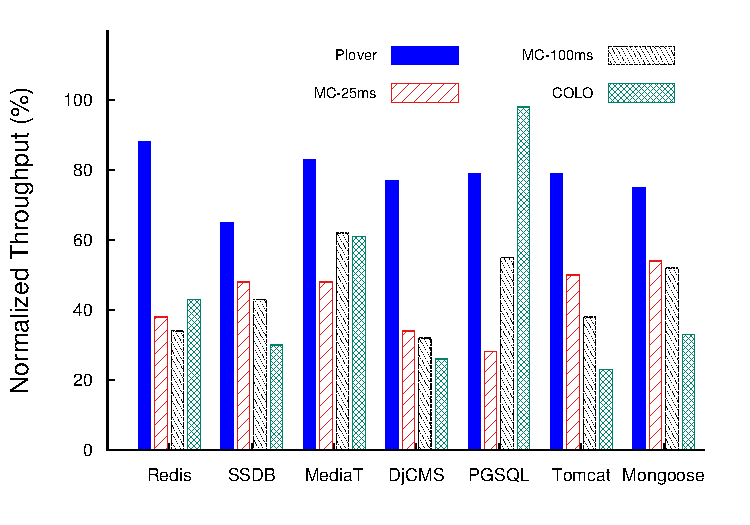
\includegraphics[width=3in]{figures/FIG1__throughput-overhead}
\caption{{\em Throughputs normalized to unreplicated executions (4 vCPUs per 
VM)}. 100\% means no overhead.}
\label{fig:vmtput}
\end{figure}

\begin{figure}[htbp]
\centering
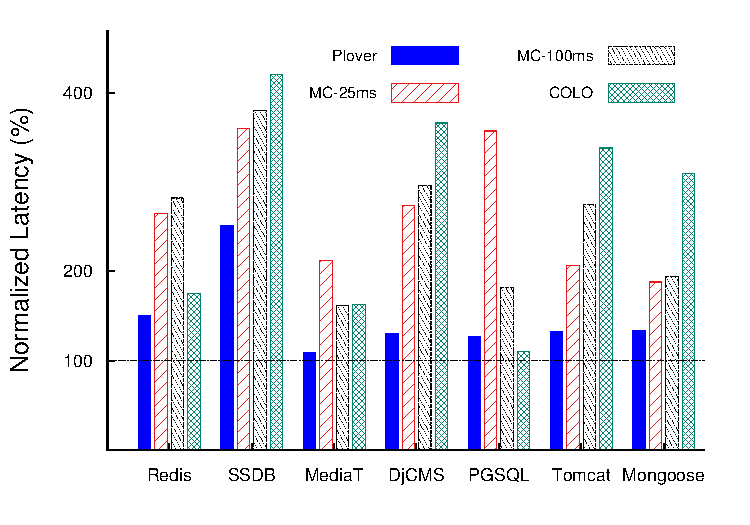
\includegraphics[width=3in]{figures/FIG9_latency-overhead}
\caption{{\em Response times normalized to unreplicated 
executions (4 vCPUs per VM)}. 100\% means no overhead.}
\label{fig:latency}
\end{figure}

For \redis and \ssdb, each request contains a batch of 1K operations 
of 50\% SET and 50\% GET; for the other five services, each request contains 
one operation. We found sending operations in batches for \redis and \ssdb made 
them reach peak throughput. For instance, when each request for \redis contains 
only one SET or GET operation, \redis's throughput is only 43K operation/s for 
32 connections; when each request is a 1K-operation batch, its throughput 
reaches a peak value of 451K operation/s for 32 connections.

We compared \yyy with two fault-tolerance systems:
QEMU-MicroCheckpoint~\cite{qemu-mc} (for short, \qemumc),  a \remus-based 
primary-backup system carried in QEMU~\cite{qemu}; and 
\colo~\cite{dong2013colo}, a primary-backup system acquired and deployed by 
Huawei~\cite{fusionsphere}. \qemumc has an RDMA 
implementation~\cite{qemu-mc-rdma}, but it is being actively developed and 
not runnable on our hosts. We did not use \remus because 
it was built before 2008 and did not run on our hosts. \colo runs the same 
service on both primary and backup, compares per-connection network outputs, 
and does a synchronization if any connection's output diverges.

Figure~\ref{fig:vmtput} shows \yyy, \qemumc, and \colo's throughput on 
7 services. All results are normalized to unreplicated executions ran 
in \kvm because the actual throughputs of different services largely vary. 
\qemumc includes results for both the 25\ms-slot (\remus's default) and 
100\ms-slot (\qemumc's default).
All experiments ran on 4-vCPU per VM (unless specified) because 
\colo~\cite{dong2013colo} and \remus~\cite{remus:nsdi08} evaluated up to 4 
vCPUs per VM. On average, \yyy's throughput is \avgtput higher than \qemumc and 
\colo.

\pgsql is the only service that \yyy is slower than \colo. \colo compares 
per-connection outputs between its primary and backup, and it 
skips transferring memory if outputs did not diverge. \pgsql ran SQL 
transaction workloads and its outputs were mostly the same. Except for 
\pgsql, \yyy was several times faster than \colo. 

To analyze \colo, we also looked into \ssdb, which 
had concurrent SET/GET requests. We found that \colo's output divergence 
was frequent when data dependencies exist among connections (\ie, GET 
requests frequently got different responses when SET and GET requests on the 
same key arrived at \ssdb concurrently). When any output in any connection 
had an output divergence, \colo did a synchronization operation. \colo 
evaluation shows that it greatly slowed down when the number of client 
connections was large. \yyy is not sensitive to outputs.

Figure~\ref{fig:latency} shows the response time of the four systems normalized 
to unreplicated executions. For five services (excluding \redis and \ssdb), 
\xxx's overhead of response time follows the same trend as the 
overhead of throughput because each client connection in these five services 
sends requests one by one. For \redis and \ssdb, because the requests arrive in 
batches in order to saturate the two services, all four systems incur 
high overhead on response time. Specifically, \yyy incurred the highest latency
overhead for \ssdb, because it had a low same dirty page rate of 
77\%. 

Figure~\ref{fig:bandwidth} explains why \yyy's performance was higher. 
\yyy consumes \avgbandwidth less bandwidth than both \qemumc
and \colo on average. This reduction makes \yyy the first VM fault-tolerance 
system that supports consolidating multiple VMs on a host.

\begin{figure}[htbp]
\centering
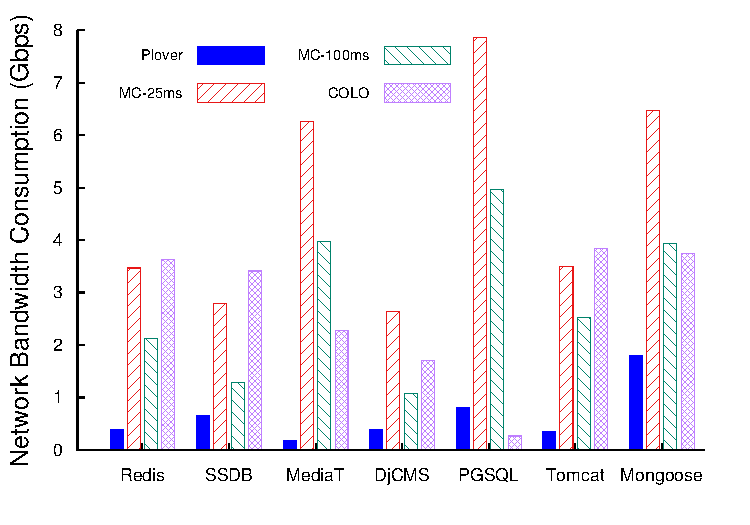
\includegraphics[width=3in]{figures/FIG2__network_bandwidth}
\caption{{\em \yyy network bandwidth consumption compared with \qemumc and 
\colo (all used four vCPUs per VM)}.}
\label{fig:bandwidth}
\end{figure}

\section{Current Status of \xxx and \yyy} \label{sec:status}
So far, we have implemented the normal case protocol of \xxx 
\section{Conclusion} \label{sec:conclusion}

\xxx is an RDMA-based \paxos system that can efficiently replicate general 
server programs. In this report, we have demonstrated the following properties 
of \xxx.

\textbf{Novel.} \xxx's runtime system uses \emph{fast} RDMA primitives to 
invoke consensus processes on requests \emph{concurrently} 
(\S\ref{sec:concurrent}). Besides, it addresses several practical issues 
including \emph{atomic} delivery of RDMA messages (\S\ref{sec:atomic}) and  
\emph{transparent} replication. All these features make \xxx a novel RDMA-based 
\paxos protocol.

\textbf{Applicable.} Our initial results in Section 
(\S\ref{sec:evaluation}) show that \xxx can provide fault tolerance to server 
programs with low performance overhead without requiring server developers' 
intervention. Compared with \nprog server programs' unreplicated executions, 
\xxx incurred \latencyoverhead overhead in response time and \tputoverhead in 
throughput. Its consensus latency outperformed four traditional consensus 
protocols by at least \comptradlow and faster than a recent RDMA-based consensus 
protocol \dare by \fasterDARE in average. This consensus latency stayed almost 
constant  to the number of replicas and concurrent requests. Furthermore, 
Section (\S\ref{sec:vm-integration}) indicates that \xxx has the potential to 
greatly improve the reliability of other applications (\eg, virtual machine) as 
well.

\end{sloppypar}

% uncomment to tweak with bib spacing
%\setlength\bibsep{2.25pt}
{
%\small
 \bibliographystyle{abbrv}
 \bibliography{bib/biblio}
}

\end{document}
